\documentclass[man,a4paper,noextraspace,apacite]{apa6}
\usepackage{apacite}

\title{Always Use Welch's t Test to Compare the Means of Two Independent Groups}
\shorttitle{Welch t Test}
\author{Joshua D. Wondra and Richard Gonzalez}
\affiliation{University of Michigan}

\abstract{When testing whether the means of two independent groups are different from each other, researchers typically use Student's t test, which assumes that the population variances of the two groups are equal. If there is reason to believe that the group variances are unequal, then researchers can use Welch's t test, which does not assume equal variances, as an alternative. We were interested in finding a simple decision rule that could be used to decide when to use Student's vs. Welch's t test. We used Monte Carlo simulations to compare the type I error rate, power, and coverage probability of Student's and Welch's t tests when testing the difference in the means of two groups across different variance ratios, sample size ratios, sample sizes, and effect sizes. We recommend the following rule: Always use Welch's t test to compare the means of two independent groups.}
\keywords{t test, new statistics, Welch}

\authornote{Joshua D. Wondra, Department of Psychology, University of Michigan.

Richard Gonzalez, Department of Psychology, University of Michigan.

Correspondence concerning this article should be addressed to Josh Wondra, Department of Psychology, University of Michigan, 530 Church St., Ann Arbor, MI 48109-1043.

Contact: jdwondra@umich.edu}


\usepackage{Sweave}
\begin{document}
\Sconcordance{concordance:WelchManuscript-MASTER.tex:WelchManuscript-MASTER.Rnw:%
1 66 1 48 0 1 85 7 1 1 16 10 1 1 16 14 1 1 20 10 1 1 4 10 1 1 4 9 %
1 1 69 9 1 2 0 11 1 2 0 4 1 1 150 1 1 1 152 11 1 1 8 6 1 1 122 2 1 %
1 122 6 1 1 0 12 1 1 7 4 1 1 225 5 1}

\maketitle

    Data analysis involves a series of decisions on the part of the researcher about which statistical test answers the research question, whether the test is suitable to the data, and whether there is an alternative test that works better. Recent discussions of false positives in psychology research \cite<e.g.,>{Fiedler2012, Ioannidis2012, Nosek2012, Simmons2011, Wagenmakers2012} highlight the tension between two valued outcomes of the decision process. On the one hand, researchers want to avoid mistakenly claiming that there is a true effect where none exists, which involves a concern with false positives. On the other hand, researchers want to find true effects where they do exist, which involves a concern with power. In addition, there is a growing concern with estimating and reporting effect sizes \cite{Cumming2014}. Some have argued that due to some common research practices, such as running underpowered studies, the effects that make it into published papers are spuriously large \cite<e.g.,>{Bakker2012, Ioannidis2008}. Researchers must find a way to balance the concerns with false positives, power, and effect size estimation as they make their decisions. 

    One of the first decisions that many researchers learn is how to compare the means of two independent groups--they run a t test. But even this basic comparison involves a choice between the classic Student's t test \cite{Student1908} or the alternative Welch-Satterthwaite test \cite{Welch1938, Satterthwaite1946}. Most researchers learn about Student's t test in the first statistics class that they ever take. When you use Student's t test to compare the means of independent groups, you make three assumptions about the populations that the data come from: 
\begin{APAenumerate}
    \item Normality: The data from each group have a normal distribution.
    \item Independence: All observations are independent of each other, meaning that the probability of one observation having a particular value does not depend on the probability of another observation having a particular value.
    \item Equal variances: The data from each group have the same variance.
\end{APAenumerate}
    
If these assumptions hold, then you can find the t-value by taking the difference in group means and dividing by the standard error of that difference:   
    \begin{equation}
    t = \frac{\overline{x}_1-\overline{x}_2}{s_{\overline{x}_1-\overline{x}_2}}
    \end{equation}
    The p-value for the value of the t statistic depends on the degrees of freedom, $df=n_1+n_2-2$. You are more likely to reject the null hypothesis and conclude that there is a difference in the group means as the t-value and the degrees of freedom get larger. This means that you are more likely to conclude that there is a difference when the sample size gets larger (which increases the degrees of freedom), when the difference in group means gets larger (which increases the numerator of t), or when the standard error gets smaller (which decreases the denominator of t). 
    
    In order to compute the standard error for the t test, you need to find the variance of the difference in group means. When the population variances of the two groups are equal, then the  variance of the difference in group means is equal to the population variance of each group. This means that if you knew the population variance of either group, then you could substitute it for the population variance of the difference in group means to compute the standard error. In practice, however, you rarely know the population variances, and instead you estimate them from the sample variances in your data. Unfortunately, even if the population variances are identical, the sample variances are rarely identical due to sampling error, so you can't substitude the sample variance of one of the groups for the variance of the difference in means to find the standard error. Student's t test deals with this problem by pooling the sample variances of the two groups into a weighted average that is used to estimate the population variance, which is assumed to be equal for the two groups and for the difference in group means. The group with the larger sample size is given more weight than the group with the smaller sample size. This means that when the bigger group has the begger variance, the standard error is bigger, but when the bigger group has the smaller variance, the standard error is smaller.

    If either the data or the study design suggests that the assumptions of normality, independence, and equal variances do not hold, then Student's t test is not the right choice and an alternative test should be used. If the group variances are unequal, then the Welch-Satterthwaite t test (hereafter called Welch's t test for the sake of brevity) is a good alternative choice. Many researchers might not have learned about Welch's t test in their formal statistical training, though most have encountered it in their analyses. For those who use SPSS to analyze their data, Welch's t test is in the "Equal variances not assumed" row that appears when they run an independent samples t test. For those who use R, Welch's t test is the default when they use the \texttt{t.test()} function and they can only get Student's t test by setting the \texttt{var.equal} argument to \texttt{TRUE}.
    
        As with Student's t test, Welch's t test assumes normality and independence; however, it does not assume that the population variances are equal. The standard error is based on separate group variances instead of a common variance. Additionally, Welch's t test decreases the degrees of freedom to the extent that the group variances are unequal. Because of these differences, the two tests can disagree about whether there is a difference in group means. Because Welch's t test decreases the degrees of freedom, it might be more conservative and less likely to reject the null hypothesis. On the one hand, this might make Welch's t test a better choice if Student's t test finds more false positives when variances are unequal. On the other hand, this might make Welch's t test a worse choice if it is not powerful enough to detect true effects. 
        
    However, Welch's t test might not always be more conservative. The power of the two tests is not only based on the degrees of freedom, but also on the standard error. This means that Welch's t test could be more powerful than Student's t test if the separate variances standard error is smaller than the pooled variances standard error. 
    
    How do you decide which test to use? The typical approach is to use Student's t test unless there is evidence that the two groups have unequal variances. The challenge is how to find that evidence. 

    One option is to run another test of the null hypothesis that the variances are equal, such as Levene's test for homogeneity, which shows up by default in SPSS, and use Welch's t test if you reject the null. However, these tests of assumptions make their own assumptions that go unchecked and they are sensitive to sample size \cite{Gonzalez2008}. In addition, simulation studies find that running tests of equal variances to decide whether to use Student's or Welch's t test is not effective \cite{Zimmerman1996,Zimmerman2004}. 

    A second option is to visualize the data using boxplots and make a judgment about whether the variances appear to differ.  With smaller sample sizes, you can tolerate larger apparent differences. This strategy can be enhanced by simulating data for two groups of that have sample sizes equal to the sample sizes in your actual data, changing whether the variances are equal or unequal, and seeing if the boxplots of your data look like the boxplots of the simulations with equal variances. 

    A third option that has not been tested to our knowledge is to examine the ratio of the degrees of freedom between Student's t test and Welch's t test. If they differ to a large extent, then it might be a sign that the group variances differ.

    A fourth option is to change the typical approach. Under ideal conditions, when variances and sample sizes are equal, Welch's t test is equivalent to Student's t test. If using Welch's t test generally leads to better decisions than Student's t test under both ideal and non-ideal conditions, then instead of using Student's t test by default it might be better to always use Welch's t test.
    
    We examined these second, third, and fourth options in a Monte Carlo simulation study. 
    
\section{Method}

    We ran Monte Carlo simulations of two independent groups with normally distributed data. We examined the type I error rate, power, and coverage probability for both Student's t test and Welch's t test under different conditions. We varied the ratio of population variances ($\sigma_{1}^2/\sigma_{2}^2$ = 1/5, 1/2, 1, 2, or 5; for each, the smaller $\sigma^2$ = 2), the sample sizes (smallest n = 20, 50, or 100), and the ratio of sample sizes ($n_{1}/n_{2}$ = 1, 2/3, or 1/2). 
    
    Additionally, we varied the difference in group means based on Cohen's d values of 0, .2, .5, and .8 when variances were equal. Importantly, Cohen's d assumes that the population variances are equal and pools the group variances just like Student's t test. This means that there is no true Cohen's d when variances are unequal. Therefore, we used the same differences in group means when variances were unequal. Because we changed the variance ratio by increasing the variance of one group, the mean differences could be considered to represent smaller effects when variances are unequal.
    
    For each condition, we set the seed to 2184 and ran 10,000 simulations. When we report conditions with equal sample sizes and variance ratios of 2 and 5, they are identical to the conditions with equal sample sizes and variance ratios of 1/2 and 1/5. 

\section{Results}   


\subsection{Visualizing Data with Boxplots} 
    One option for deciding whether the group variances are equal is to examine boxplots. Figure 1 displays boxplots from simulations of two groups with equal variances (top) and from simulations of two groups with unequal variances where the variance of the group to the right is five times as large as the variance of the group to the left (bottom). The first row of each set of boxplots displays groups with $n$ = 20 and the second row displays groups with $n$ = 100. The population distributions are displayed above the boxplots. When the sample sizes are smaller there is more variability in the boxplots. Seeing some variability in the spread of the groups is normal, even when the population variances are equal. In contrast, when sample sizes are larger there is more consistency in the boxplots. Smaller differences in the spread of the boxplots might be a sign that the population variances differ when $n$ = 100. By examining several additional simulations it would be possible to see how much variability in the boxplots is normal when variances are equal or unequal.
   
\begin{figure}
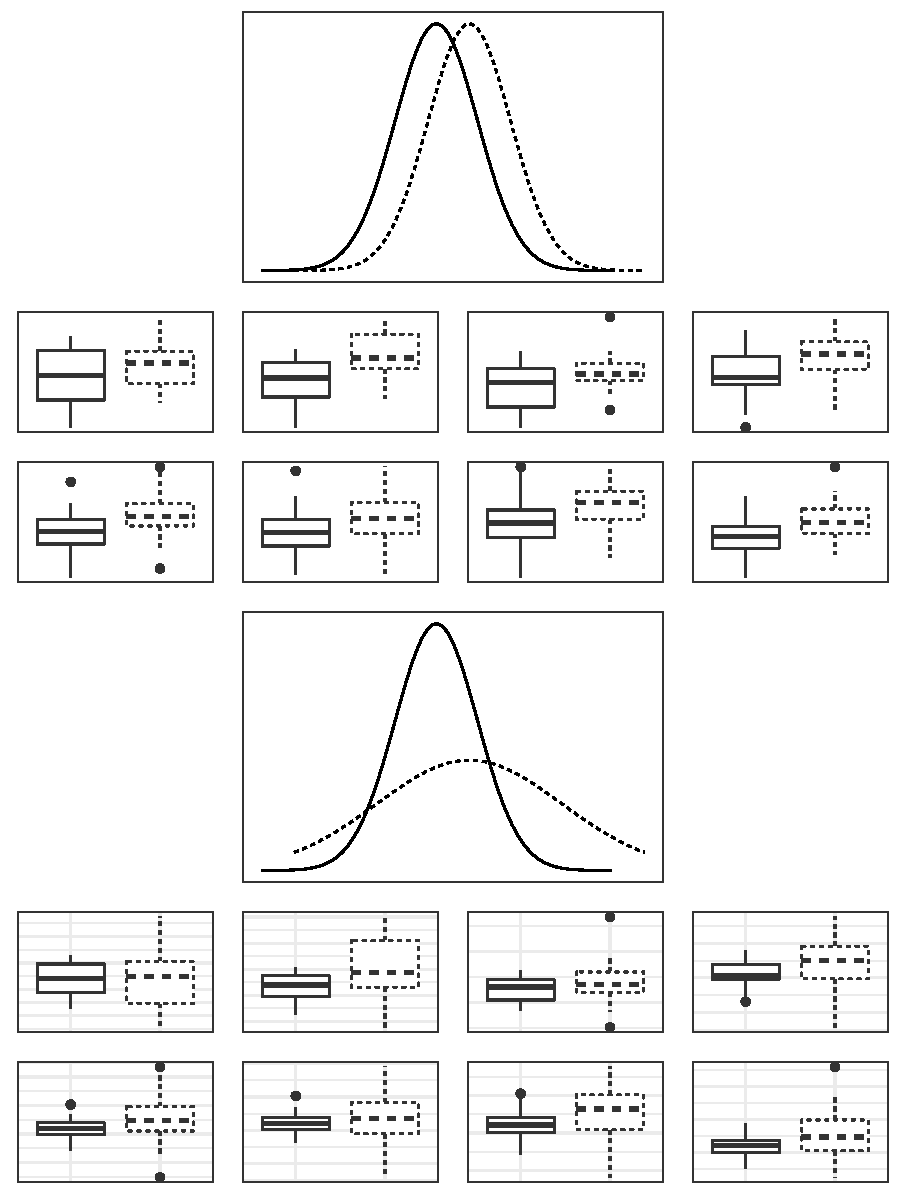
\includegraphics{WelchManuscript-MASTER-varEqualBoxplots}

\textit{Figure 1.} Boxplots for groups with equal variances (top) and unequal variances (bottom). For each set of boxplots, the first row displays groups with $n$=20 and the second row displays groups with $n$=100.
\end{figure}

\subsection{Does the df Ratio Help?}
    We examined whether looking at the ratio of the degrees of freedom (df) from Welch's t test to the df of Student's t test could provide a heuristic for deciding that the group variances are unequal. Rather than simulate the df ratio, we used the analytical formulas for the two dfs to see how the df ratio should change as the population variances and the sample size ratio change.

    The top graph in Figure 2 displays the change in the df ratio as the variance ratio increases when sample sizes are equal. As expected, the ratio decreases as the difference in variances grows larger. When the variances are equal, the df ratio is equal to one (though in real data, the sample variances will rarely be exactly equal even if the population variances are equal). When the variance of one group is double the variance of the other, the ratio drops to .9. A useful heuristic might be to assume that the variances are unequal when the ratio falls below 96\%.
  
\begin{figure}
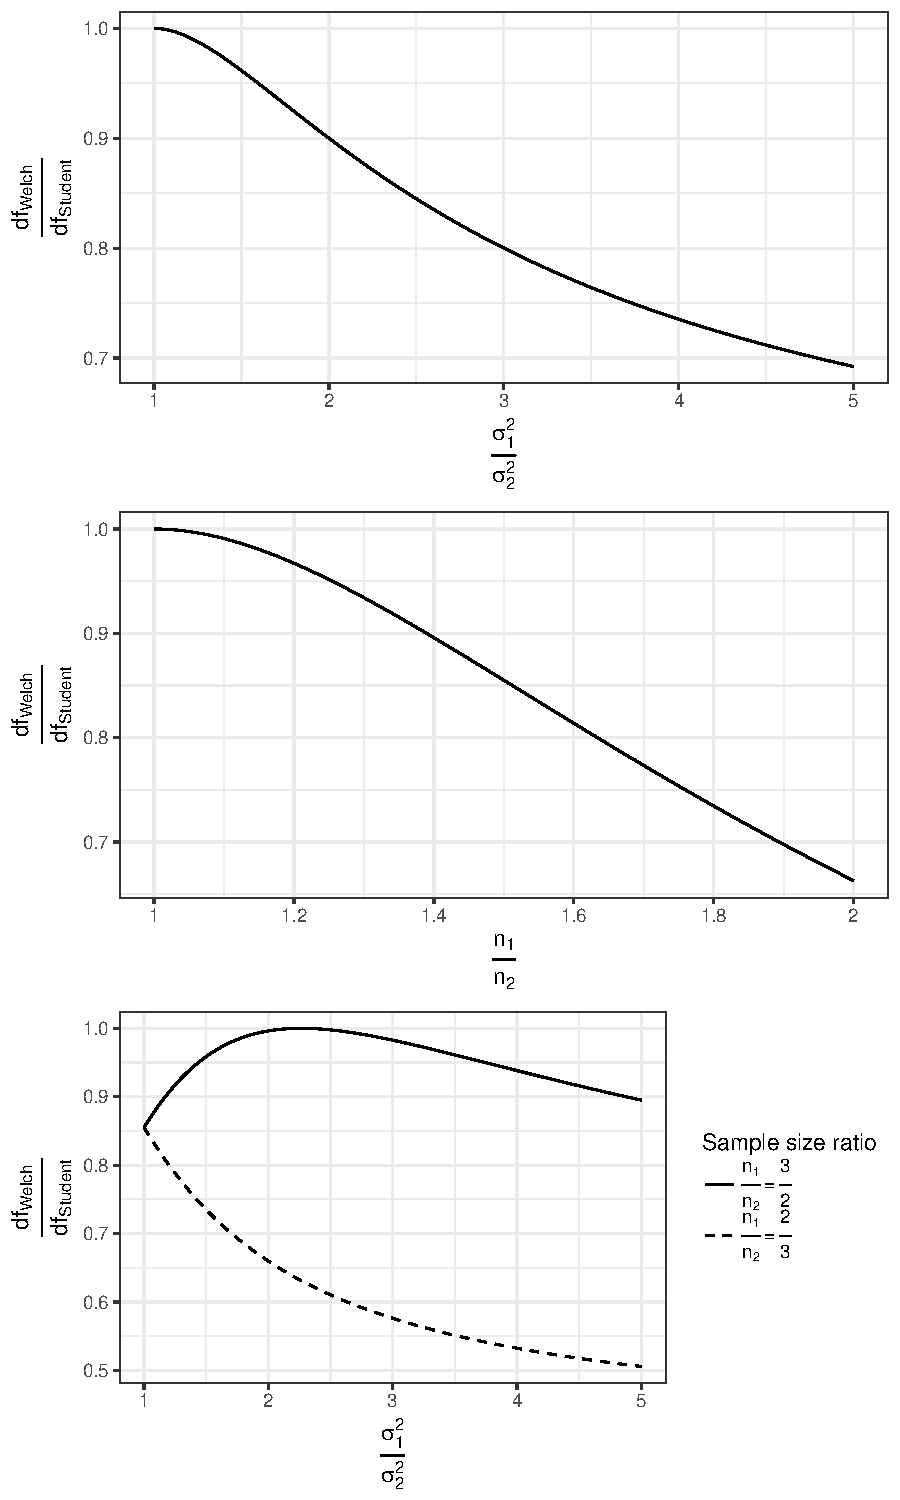
\includegraphics{WelchManuscript-MASTER-dfratiosDiffvars}

\textit{Figure 2.} Degrees of freedom ratio when sample sizes are unequal and variances are equal (top), when variances are equal and sample sizes are unequal (middle), and when both variances and sample sizes are unequal (bottom).
\end{figure}

    But now look at what happens when the variances are equal and the sample size ratio changes (middle graph of Figure 2). Even though the variances stay the same, the df ratio decreases as the difference in sample sizes grows larger. The 96\% heuristic would lead us astray and we would incorrectly conclude that the variances are unequal when only the sample sizes are unequal.

%' \begin{figure}
%' <<dfratiosDiffNratios, echo=FALSE,  collapse=TRUE, fig=TRUE>>=
%' 
%' ggplot(data.frame(x=seq(50,100,.1)), aes(x)) + 
%'     stat_function(fun=partial.df(var='n2', params=list('n1'=50,'n2'=50,'var1'=2,'var2'=2))) +
%'     labs(y=bquote(frac('df'['Welch'],'df'['Student'])), x=bquote(frac('n'[1],'n'[2]))) +
%'     scale_x_continuous(breaks=c(50,60,70,80,90,100), labels=c(50,60,70,80,90,100)/50)
%' 
%' @
%' 
%' \textit{Figure 4.} Degrees of freedom ratio when sample sizes are unequal and variances are equal.
%' \end{figure}

    The picture becomes even more complicated when both the sample sizes and the variances are unequal (bottom of Figure 2). In this case, the effect of different variances on the df ratio depends on whether the larger group has the larger variance or the smaller variance. As the variance of the smaller group increases, the immediate drop in the df ratio is quite dramatic before it begins to level off. However, as the variance of the larger group increases, the move from equal to unequal variances actual counteracts the effect of the unequal sample sizes at first, and the df ratio approaches one before it drops again. Due to the difference in sample sizes, a 96\% heuristic would mislead us into concluding that variances are equal when they are actually 2-3 times different from each other.  

%' \begin{figure}
%' <<dfratiosDiffvarsDiffNratios, echo=FALSE,  collapse=TRUE, fig=TRUE>>=
%' ggplot(data.frame(x=seq(2,10,.1)), aes(x)) + 
%'     stat_function(fun=partial.df(var='var2', params=list('n1'=75,'n2'=50,'var1'=2,'var2'=2)), aes(colour='n2')) +
%'     stat_function(fun=partial.df(var='var2', params=list('n1'=50,'n2'=75,'var1'=2,'var2'=2)), aes(colour='n1/2')) +
%'     scale_colour_manual(values=c('blue', 'red'), labels=c(bquote(frac('n'[1],'n'[2])~'='~frac(3,2)), bquote(frac('n'[1],'n'[2])~'= '~frac(2,3)))) +
%'     labs(y=bquote(frac('df'['Welch'],'df'['Student'])), x=bquote(frac(sigma[1]^2,sigma[2]^2))) +
%'     scale_x_continuous(breaks=c(2,4,6,8,10), labels=c(2,4,6,8,10)/2)
%' @
%' 
%' \textit{Figure 5.} Degrees of freedom ratio when sample sizes are unequal and variances are unequal.
%' \end{figure}

In short, the usefulness of a heuristic based on the df ratio is limited to cases when the sample sizes are equal. 

\subsection{When Does Each Test Perform Best?}
    There does not seem to be a simple rule based on the df ratio to detect whether variances are unequal, so we decided to examine when the Welch and Student t tests would perform best based on the sample size, variance ratio, and sample size ratio. We examined how well each test balances concerns with false positives, power, and estimation. Some prior research has examined the Type I error rate for the two tests \cite{Boneau1960, Zimmerman1993, Zimmerman2004, Zimmerman1996, Zimmerman2009} and some has also examined the power of the two tests, though not with the complete configuration of conditions that we examined in our simulations \cite{Neuhauser2002, Zimmerman1993}. Nevertheless, we believe that it will be informative to display the false positives and power of the two tests here. We also discuss implications for effect size estimation, which follows from the false positive results but has not, to our knowledge, been discussed explicitly in past research.
    
\subsubsection{Type I Error Rates}

    The expected type I error rate is $\alpha = .05$. The observed type I error rate for Student's t test remained close to the expected .05 rate when either the sample size or the population variances were equal, but it varied widely when both population variances and sample sizes were unequal (see Figure 3). When the group with the larger sample size had the larger variance (the left side of the top graph in Figure 3), the type I error rate dropped as low as about .01, but when the group with the larger sample size had the smaller variance (the right side of the top graph in Figure 3), the type I error rate rose as high as .12, which is more than double the normally accepted false positive rate. In contrast, the observed type I error rate for Welch's t test remained close to the expected .05 rate across all conditions. Overall, Welch's t test consistently behaved as expected when it comes to false positives. Student's t test did not.

\begin{figure}    
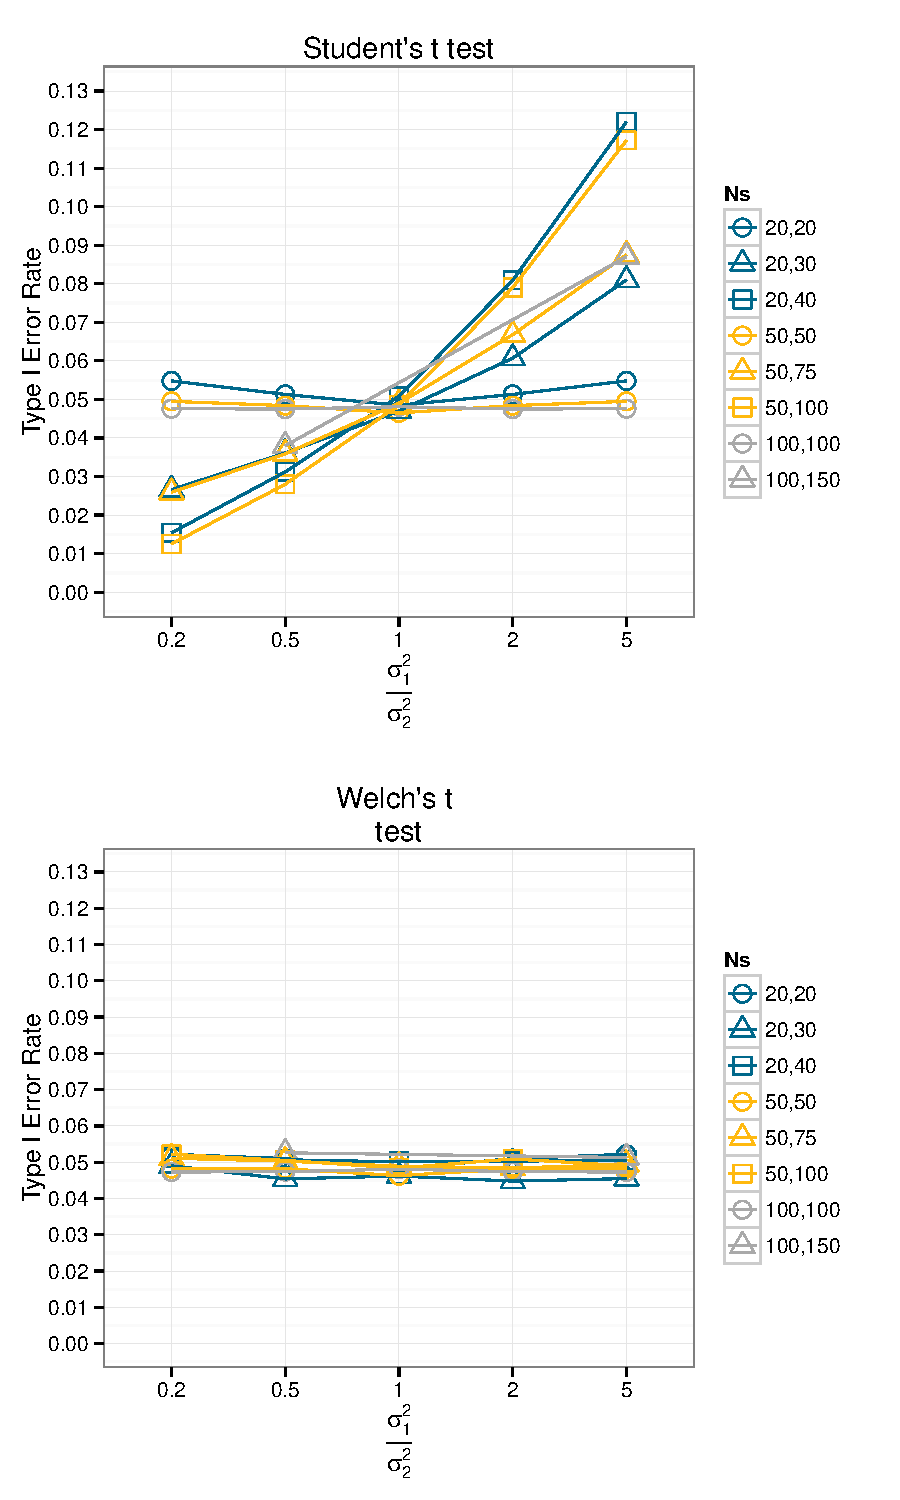
\includegraphics{WelchManuscript-MASTER-Type1ClassicPlot}

\textit{Figure 3.} Type I error rates for Student's t test and Welch's t test as the variance ratio, sample size ratio, and sample sizes vary.
\end{figure}


%' \begin{figure}
%' <<Type1WelchPlot, echo=FALSE, fig=TRUE>>=
%' T1welch
%' @
%' 
%' \textit{Figure 8.} Type I error rates for Welch's t test.
%' \end{figure}

\subsubsection{Power}



    Is Welch's t test underpowered compared to Student's t test? Figure 4 displays the power of the two tests to detect small, medium, and large effects under the different conditions. For both tests, power decreased as variances became unequal because we increased one group's variance; however, the power of each test decreased at a different rate depending on the sample size and variance ratios. Figure 5 displays the difference in power between Student's t test and Welch's t test, with higher numbers indicating that Student's t test is more powerful. When the sample sizes or variances are equal, the power of the two tests is approximately equal. However, when both the sample sizes and variances are unequal, there are differences in power. Overall, Student's t test is more powerful when the large sample has the smaller variance, whereas Welch's t test is more powerful when the small sample has the smaller variance. These differences are the most dramatic when one sample is twice the size of the other. 
    
    The conditions in which Student's t test has the greatest power over Welch's t test, when one sample is twice the size of the other and the large sample has the small variance, are the same conditions in which Student's t test has a risk of doubling the false positive rate. Whatever advantage Student's t test has in terms of power is undermined by the inflated false positive rate. In contrast, in the conditions where Welch's t test was more powerful, it never inflated the type I error rate beyond the expected rate. These results support the decision to always use Welch's t test. By using Welch's t test, you sometimes have greater power to detect true effects, but you don't have to worry about sacrificing concerns with false positives.  

\begin{figure}
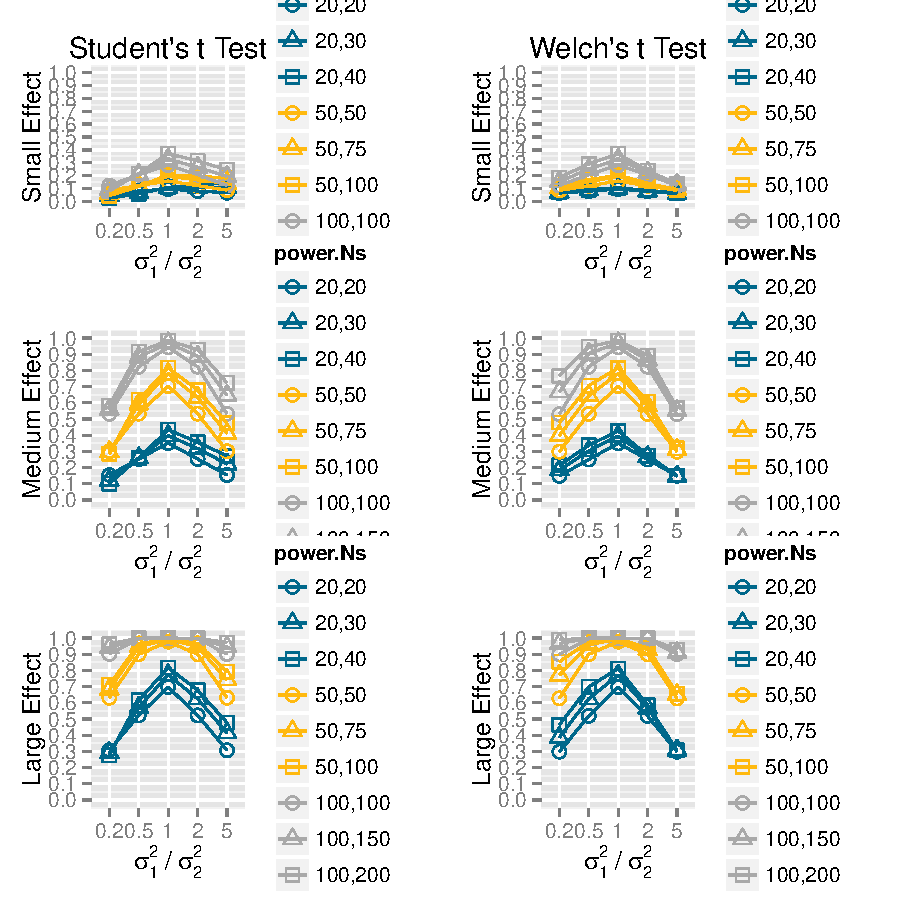
\includegraphics{WelchManuscript-MASTER-plotPower}

\textit{Figure 4.} Power of Student's and Welch's t tests.
\end{figure}

\begin{figure}
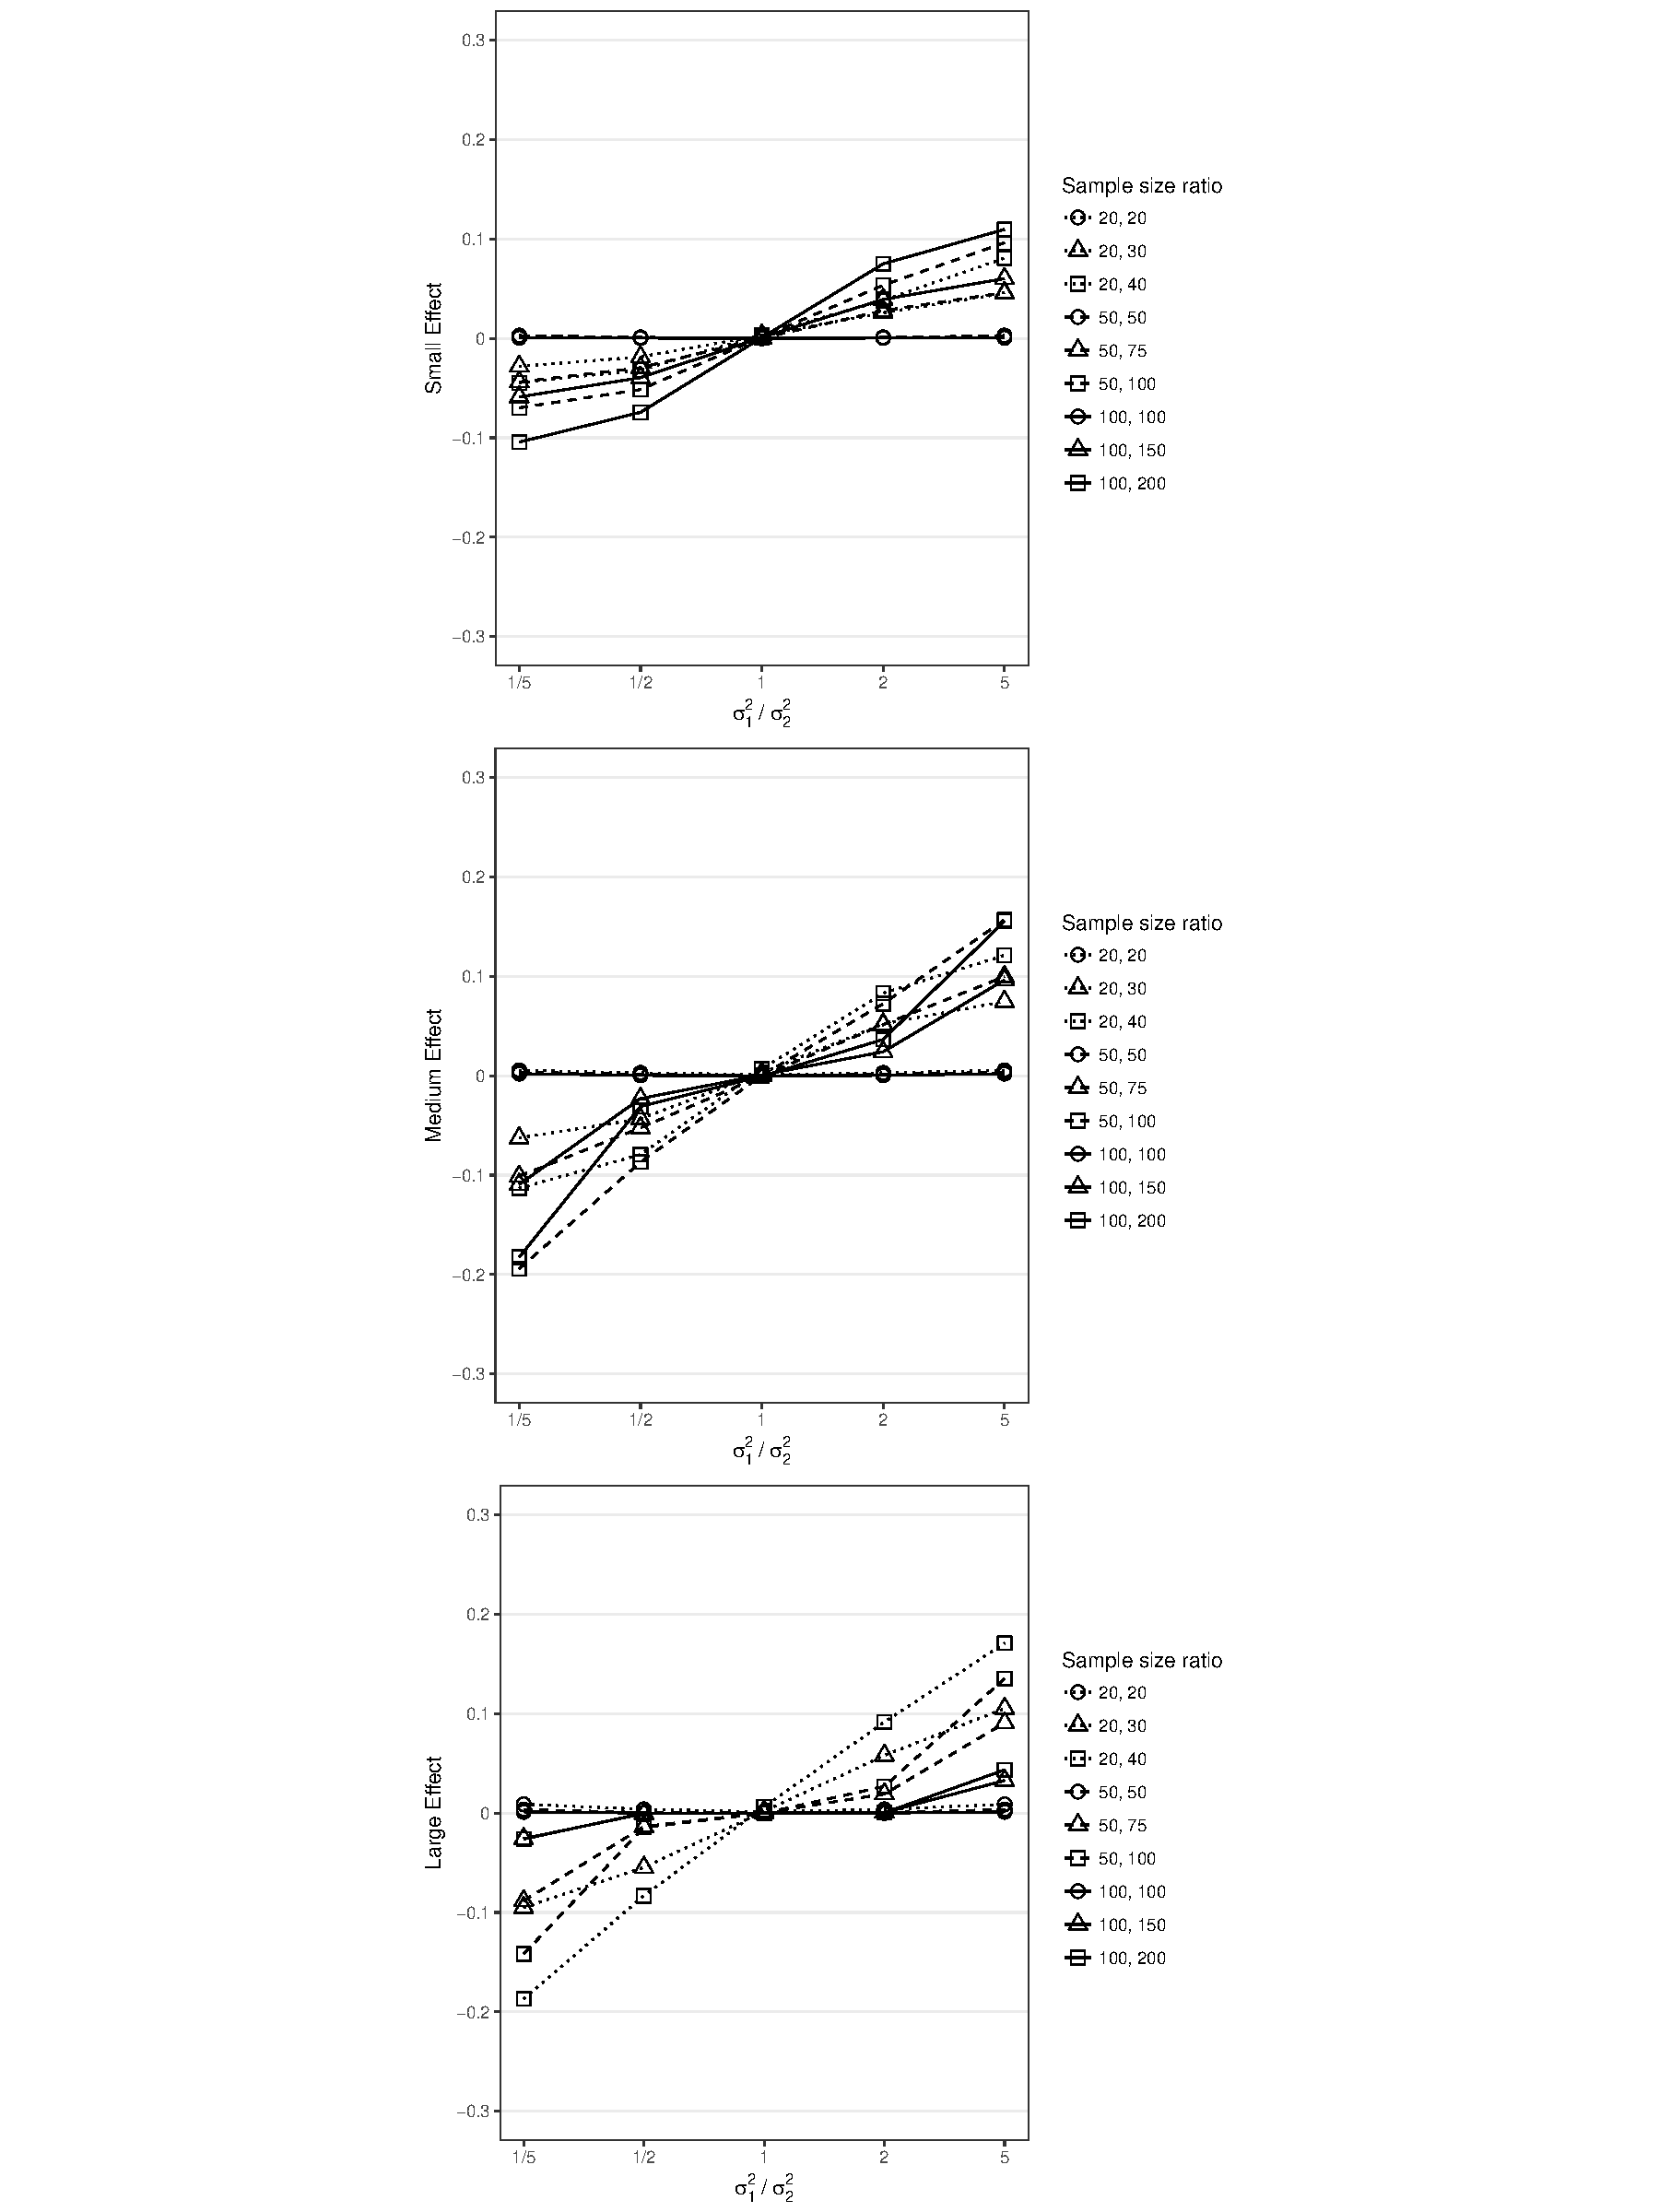
\includegraphics{WelchManuscript-MASTER-plotPowerDiff}

\textit{Figure 5.} Difference in the Power of Student's and Welch's t tests (Student-Welch).
\end{figure}

\subsubsection{Coverage Probability}
We examined the coverage probability of 95\% confidence intervals constructed using Student's t test and Welch's t test. Coverage probability refers to the proportion of confidence intervals that contain the true population value of the estimated parameter, which is the difference in group means in this case. For 95\% confidence intervals, by definition the expected coverage probability is .95. Because the coverage probability of a confidence interval is not influenced by the effect size, we only show the coverage probabilities when the null hypothesis is true. Additionally, when the null hypothesis is true and $\alpha = .05$, the coverage probability of 95\% confidence intervals has a simple relationship with the type I error rate--the coverage probability is the complement of the type I error rate. Figure 6 displays the coverage probabilities of the two t tests. The coverage probability for Student's t test varies dramatically, just as the type I error rate did. When Student's t test is the least powerful, it is the most accurate at estimating the difference in means. When it is the most powerful, it is also the least accurate, and what you would believe is a 95\% confidence interval drops to as low as an 88\% confidence interval in reality. In contrast, Welch's t test performs as expected and the confidence interval contains the true effect 95\% of the time regardless of the variance and sample size ratios. 




\begin{figure}
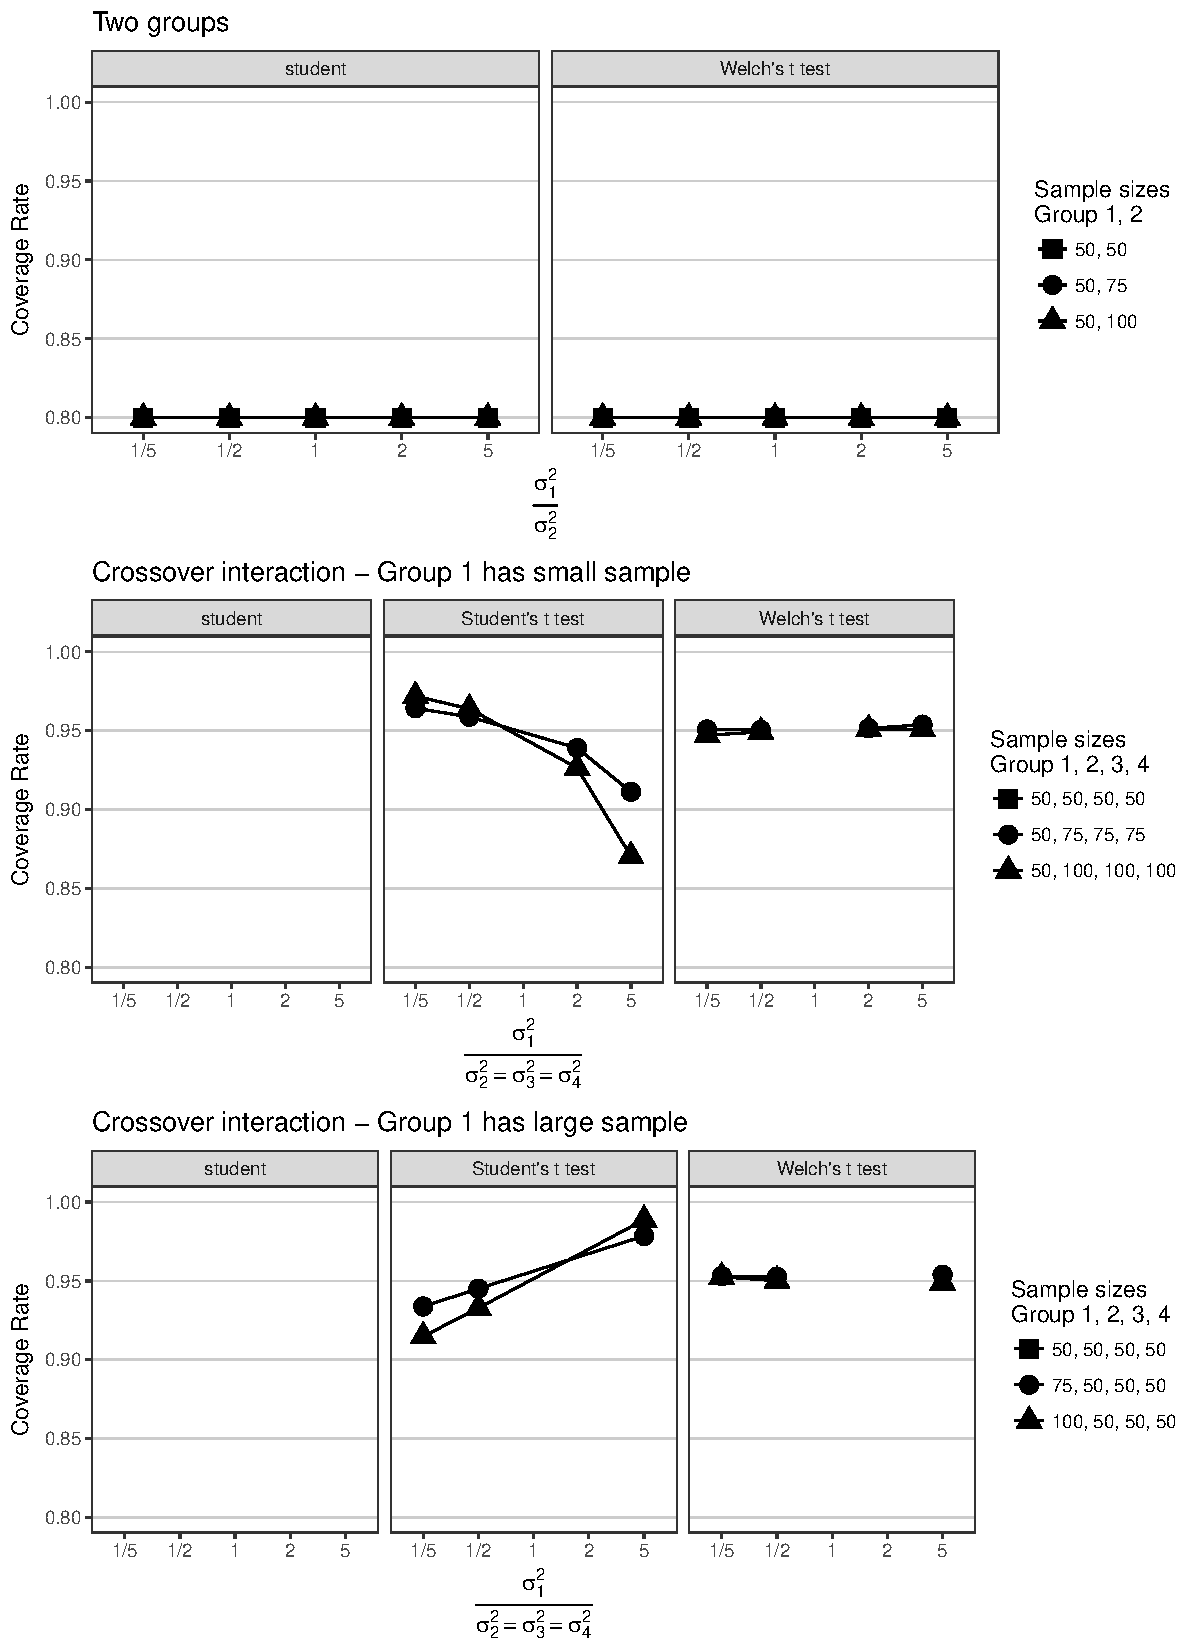
\includegraphics{WelchManuscript-MASTER-CoveragePlots}

\textit{Figure 6.} Coverage probabilities for Student's and Welch's t tests.
\end{figure}

\section{Discussion}
    We set out to find a simple rule to help researchers decide when to use Student's t test and when to use Welch's t test. We believe that the simplest rule is to always use Welch's t test to compare the means of independent groups.
    
    The results of our simulations demonstrated that when the population variances or sample sizes were equal, using Welch's t test instead of Student's t test didn't hurt. Figures 1 shows that the Welch degrees of freedom could drop below 70\% the Student's t test degrees of freedom when only the variance ratio or the sample size ratio changed. Nevertheless, the false positive rates, power, and coverage probabilities of the two tests were almost identical under these conditions. The difference in the degrees of freedom of the two tests was not very important at all. We illustrate this point in Figure 7, which shows two overlapping t distributions, one with half the degrees of freedom of the other. The tails of the distribution with the smaller degrees of freedom are a little larger than the tails of the distribution with greater degrees of freedom, but not by much. Given the same t-value, in the majority of cases these distributions would agree about whether or not to reject the null hypothesis. 
    
\begin{figure}  
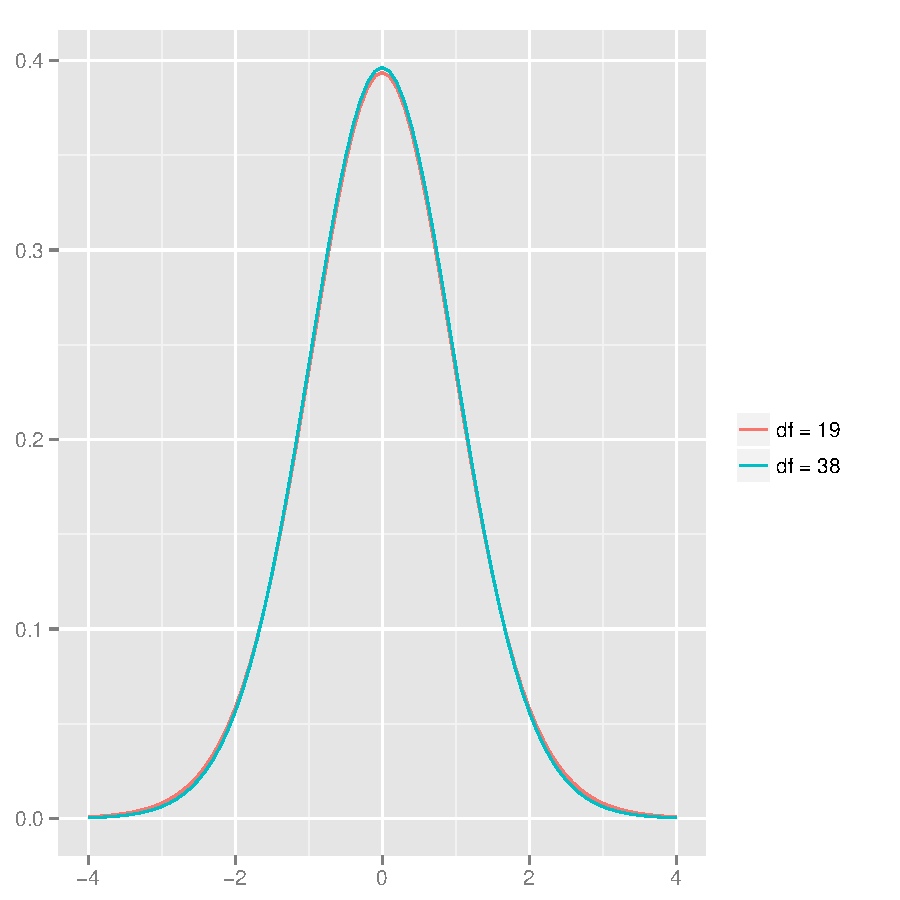
\includegraphics{WelchManuscript-MASTER-tdist}

\textit{Figure 7. Two t distributions with different degrees of freedom.}
\end{figure}
    
    More important than the degrees of freedom is the standard error, which affects the t-value itself. When either the variances or the sample sizes are equal, the pooled standard error of Student's t test and the separate variances standard error of Welch's t test are identical, and the two tests will generally agree with each other. However, when both the variances and the sample sizes are unequal, the pooled standard error of Student's t test gives more weight to the group with the larger sample size, as has been discussed by others \cite<e.g.,>{Coombs1996,Zimmerman2009}; if that group has the larger variance, then Student's t test becomes more conservative, but if that group has the smaller variance, then Student's t test becomes more liberal. In contrast, Welch's t test was more stable, regardless of which sample had the larger variance. This can be seen in Figures 3 and 6, where the type I error rate and coverage probability vary widely for Student's t test, but remain stable for Welch's t test.
    
    The biggest benefit of Student's t test was that it had more power than Welch's t test to detect true effects when the larger sample had the smaller variance--yet under these same conditions, it had an inflated type I error rate and the lowest coverage probability. Far from being underpowered, Welch's t test was more powerful than Student's t test when the larger sample had the larger variance, but under these same conditions it retained the expected type I error rate and coverage probability. Overall, Welch's t test did a better job of balancing researcher concerns about false positives, power, and estimation.
    
    We believe that researchers are more likely to use simple decision rules, and so we echo the recommendations of previous researchers to always use Welch's t test \cite{Zimmerman1996,Moser1992,Moser1989}. For researchers who insist on using Student's t test, if they run experiments, then there is some good news. With experiments, subjects are usually assigned evenly to conditions, and when sample sizes are equal the two tests perform equally well. However, for those whose research involves comparing pre-existing groups, it might not be possible to have equal sample sizes. Welch's t test is likely to outperform Student's t test because the sample variances are unlikely to be exactly equal. If a researcher still prefers a complex rule where using Student's t test is still possible, then one option is to look at boxplots to determine whether it is reasonable to assume that the group variances are equal. This judgment will be easier if the sample sizes are large. Nevertheless, researchers should rest assured that they won't suffer from using the simple rule to always use Welch's t test.
    
    We examined whether the ratio of the degrees of freedom from Welch's t test to the degrees of freedom from Student's t test could provide a good heuristic to determine whether or not the group variances are unequal. The rule had the greatest potential when it mattered the least--when the sample sizes of the two groups were equal. When the sample sizes were unequal, the degrees of freedom ratio was not a reliable indicator of unequal variances. It could become very high as variances became unequal and it could drop very low when the variances were equal. There seems to be no simple rule for deciding between the two tests based on the ratio of the degrees of freedom. Fortunately, the rule to always use Welch's t test is simpler and more effective.
    
    We note that aside from Welch's t test, there have been Bayesian approaches to the problem of comparing groups with unequal variances. \citeA[p.~104-109]{Box1973} presented analytical Bayesian t tests when equal variances is assumed and when equal variances is not assumed. When noninformative locally uniform priors are used for the group means and the logarithm of the group standard deviations, and equal variances is assumed, their solution is identical to Student's t test. When the same priors are used, but equal variances are not assumed, their solution is similar to Welch's t test, but slightly more conservative because the degrees of freedom are generally lower and the standard error is generally larger or equal. More recently, \citeA{Kruschke2013} presented a Bayesian approach to comparing group means that uses Markov Chain Monte Carlo simulations. This approach simulates the posterior distribution of means for each group based on the prior distributions and the data. For each simulation, the difference in the simulated group means is taken, which produces a posterior distribution of the difference in group means. Inferences about the difference in group means are based on this posterior distribution. Because this method does not use a t-statistic, there is no need to create a standard error for the difference in group means. 
    
    Prior simulation work comparing Student's t test to Welch's t test has focused on null hypothesis significance testing by emphasizing type I errors and power \cite{Boneau1960, Neuhauser2002, Zimmerman1993, Zimmerman2004, Zimmerman1996, Zimmerman2009}, but there important implications of this work for effect size estimation as well. Some have called for researchers to report effect sizes and confidence intervals to address some of the limitations of just reporting null hypothesis significance tests. It is important to remember that effect size estimation can also involves assumptions about group variances.
    
    We found that using Student's t test to estimate the differences in group means, which involves the assumption that the group variances are equal, had a big impact on accuracy. Under some conditions, the confidence intervals were less accurate than expected because they were too narrow, and under other conditions, they were more accurate than expected because they were too wide. Using Welch's t test, which does not assume that group variances are equal, led to more stable estimation across conditions.
    
    Cohen's d \cite{Cohen1992} is the most popular effect size for reporting the difference in two group means. It standardizes the difference based on a common standard deviation of the population--but what if there is no common standard deviation of the population? This is exactly the situation we're faced with when lifting the equal variances assumption. Because Cohen's d assumes that the group variances are equal, letting go of equal variances also means letting go of Cohen's d. 
    
    Standardized effect sizes such as Cohen's d are often desirable for their use in meta-analysis or other attempts to summarize the size of an effect based on a comprehensive body of research. But their convenience shouldn't be reason enough to brush off Welch's t test for Cohen's d, because the equal variances problem applies equally to meta-analysis. Using Cohen's d as the basis for a meta-analysis involves an implicit assumption that the group variances across the body of research are equal, an assumption which might be untenable in many cases. Potential differences in group variances might not just be a nuisance that gets in the way of building a comprehensive area of study, but they might actually be an interesting part of the effect for meta-analysts to examine. 
    
    The good news is that effect sizes are not just standardized differences in means, but they also include things like the raw difference in means \cite{Cumming2014, Kelley2012}, and confidence intervals around raw differences in means based on separate variances are easy to find. They are included in the default output of data analysis programs such as SPSS and R. Reporting descriptive statistics in their original scale might be a better practice than reporting only standardized effect sizes anyway. Reporting the raw descriptives has a few advantages. First, it does not require the researcher to commit to an equal variances assumption. Second, it provides all of the necessary information for others who want to assume equal variances to find Cohen's d, or a number of the alternatives that have been recommended \cite{Peng2013, Grissom2001}. Third, it allows other researchers to examine whether differences in group variances are a consistent part of an effect, which would be lost by just reporting the standardized difference.

    We suspect that most statistics courses in psychology teach Student's t test thoroughly and only briefly touch on Welch's t test, if they teach it at all. Indeed, we have heard colleagues who have used Welch's t test in a manuscript complain about reviewers who were suspicious when they reported degrees of freedom with decimals. These reviewers must not have learned that degrees of freedom with decimals are the norm for Welch's t test. The emphasis on Student's t test in teaching is consistent with the common strategy to start out by assuming that variances are equal and to only use Welch's t test as a back-up when the assumption has been violated. But why should we spend so much time on the equal variances assumption in the first place? Why not teach Welch's test as a safe first step that will do just fine without imposing restrictive assumptions? Student's t test could still be taught briefly so that students understand the existing literature, but we believe it would be beneficial to emphasize Welch's t test as the default approach. As demonstrated in our simulations, this approach will help lead to better decision-making when it comes to analyzing data. 




%' \begin{figure}
%' <<varDifferentBoxplots, echo=FALSE, fig=TRUE>>=
%' 
%' x1 <- seq(0,12,.1)
%' y1 <- dnorm(x1, mean=6, sd=sqrt(2))
%' x2 <- seq(1.13,13.13,.1)
%' y2 <- dnorm(x2, mean=7.13, sd=sqrt(10))
%' 
%' x <- c(x1,x2)
%' y <- c(y1,y2)
%' group <- factor(c(rep(1,length(x1)), rep(2,length(x2))))
%' 
%' ve.distributions <- qplot(x=x, y=y, fill=group, colour=group, geom='line', xlab=NULL, ylab=NULL) + geom_vline(xintercept=as.numeric(by(x,group,mean))) + theme(legend.position='none')
%' 
%' set.seed(2184)
%' ve.bplots <- c(list(ve.distributions), 
%'                lapply(1:4, function(x){
%'                  qplot(x=factor(rep(c(1,2), each=20)), 
%'                        y=c(rnorm(20,6,sqrt(2)),rnorm(20,7.13,sqrt(10))), 
%'                        geom='boxplot', 
%'                        colour=factor(rep(c(1,2), each=20)), 
%'                        xlab=NULL, 
%'                        ylab=NULL, 
%'                        ylim=c(-3,18)) + 
%'                    theme(legend.position='none', axis.text.x=element_blank())}), 
%'                lapply(1:4, function(x){
%'                  qplot(x=factor(rep(c(1,2), each=100)), 
%'                        y=c(rnorm(100,6,sqrt(2)),rnorm(100,7.13,sqrt(10))), 
%'                        geom='boxplot', 
%'                        colour=factor(rep(c(1,2), each=100)), 
%'                        xlab=NULL, 
%'                        ylab=NULL, 
%'                        ylim=c(-3,18)) + 
%'                    theme(legend.position='none', axis.text.x=element_blank())}))
%' 
%' layout <- matrix(c(0,1,1,0,2,3,4,5,6,7,8,9), nrow=3, byrow=TRUE)
%' multiplot(plotlist=ve.bplots, layout=layout)
%' 
%' @
%' 
%' \textit{Figure 2.} Boxplots for groups with unequal variances. The first row displays groups with $n$=20 and the second row displays groups with $n$=100.
%' \end{figure}


\bibliography{bibliography}
\bibliographystyle{apacite}

\end{document}
